
\section{Arquitectura PEMEA}

El proyecto PEMEA (Pan-European Mobile Emergency Apps) es una
 inciativa de la unión europea para unificar en una aplicación, la conexión 
con todos los centros de emergencia 112.

El objetivo de este proyecto es proporcionar una arquitectura que permita
 acceder a los servicios de emergencia en cualquier lugar de Europa y un 
endpoing para poder dar acceso a información ampliada del usuario, como
 por ejemplo, a su geolocalización.

El proyecto aún no esta terminado, actualmente esta en fase de pruebas.
 El inicio de la fase 2 esta planificado a principios de Septiembre 2019.

En la siguiente imagen vemos como funciona esta arquitectura.

\begin{figure}[h]
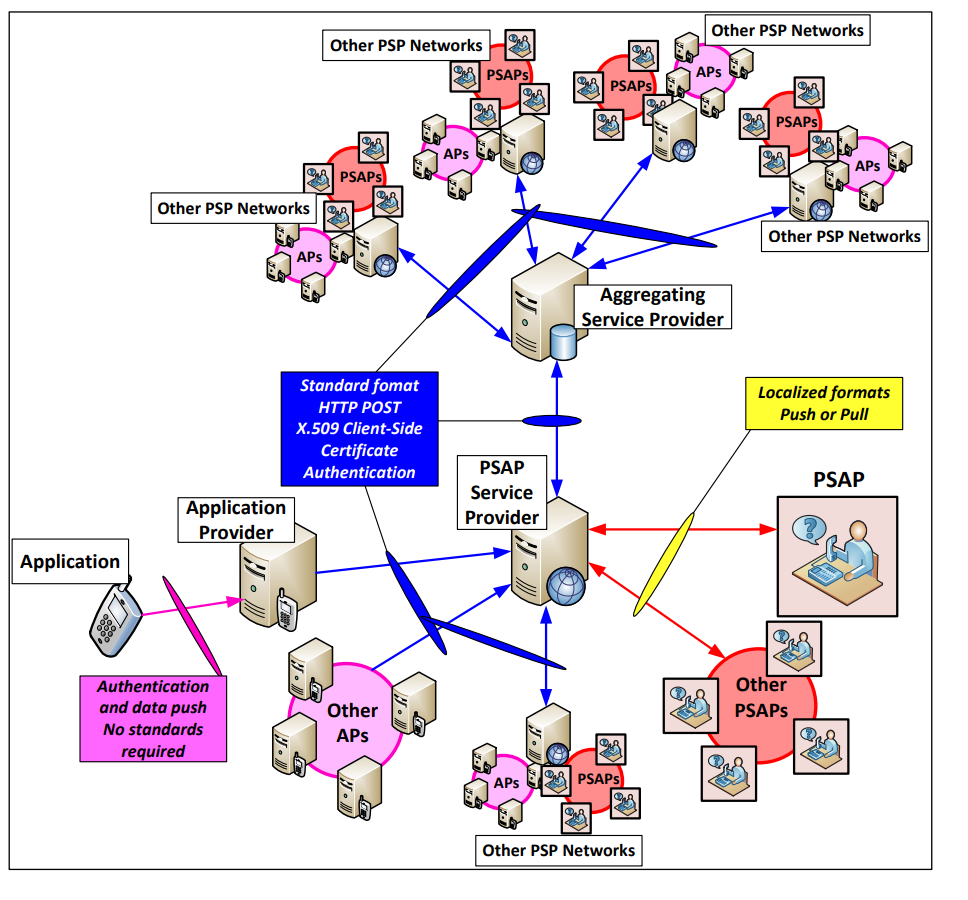
\includegraphics[scale=0.5]{pemea_arq.png} 
\caption{Arquitectura PEMEA completa.}
\end{figure}

Fuente: PEMEA~\cite{PEMEA}.